
	\begin{wrapfigure}{r}{0.34\textwidth}
\vspace{-5mm}
	% \begin{figure}[t] %插入图片
		\centering %图片居中
		\resizebox{.32\columnwidth}{!}{  %用于修改图片大小
\centering
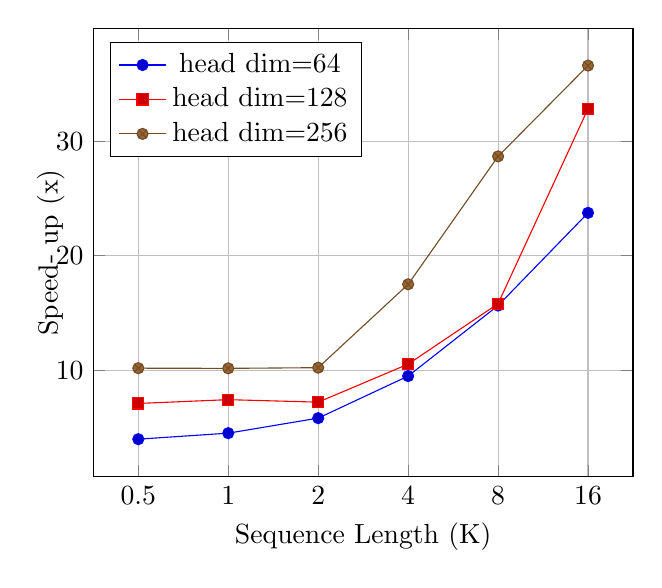
\begin{tikzpicture}
    \begin{axis}[
        title={},
        xlabel={Sequence Length (K)},
        ylabel={Speed- up (x)},
        ylabel style={yshift=-10pt},
        legend pos=north west,
        grid=both,
        xtick={512, 1024, 2048, 4096, 8192, 16384},
        xticklabels={0.5, 1, 2, 4, 8, 16},
        log ticks with fixed point,
        xmode=log,
        % ymode=log
    ]
    
    % head dim=64
    \addplot coordinates {
        (512, 10.7097 / 2.6930)
        (1024, 10.9562 / 2.4330)
        (2048, 14.0425 / 2.4151)
        (4096, 24.4682 / 2.5787)
        (8192, 47.6885 / 3.0478)
        (16384, 94.9672 / 4.0006)
    };
    \addlegendentry{head dim=64}
    
    % head dim=128
    \addplot coordinates {
        (512, 18.8856 / 2.6611)
        (1024, 19.6152 / 2.6409)
        (2048, 19.0975 / 2.6484)
        (4096, 31.2284 / 2.9655)
        (8192, 60.9088 / 3.8531)
        (16384, 191.4909 / 5.8325)
    };
    \addlegendentry{head dim=128}
    
    % head dim=256
    \addplot coordinates {
        (512, 47.2460 / 4.6427)
        (1024, 47.4189 / 4.6667)
        (2048, 47.8577 / 4.6824)
        (4096, 83.5260 / 4.7730)
        (8192, 166.8563 / 5.8201)
        (16384, 330.6606 / 9.0348)
    };
    \addlegendentry{head dim=256}
    
    \end{axis}
\end{tikzpicture}
  }
    \vspace{-1mm}
		% \caption{The x-axis is the model dimension and the y-axis is accuracy on MQAR.} 
	\caption{{Speed-up of the chunkwise parallel form vs. the recurrent form.}} 		\label{fig:kernel_speed} 
    \vspace{-5mm}
	% \end{figure}/
	\end{wrapfigure}
